\section{\texorpdfstring{$x_F$}{xF} bins}
\label{sec:a3_xFbin}
\begin{figure}[h]
	\centering
	\begin{subfigure}{0.4\linewidth}
		\includegraphics[width=0.9\linewidth]{massfit/run2-3/LH2/xF/LH2_xFbin0}
	\end{subfigure}
	\begin{subfigure}{0.4\linewidth}
		\includegraphics[width=0.9\linewidth]{massfit/run2-3/LD2/xF/LD2_xFbin0}
	\end{subfigure}\\
	\begin{subfigure}{0.4\linewidth}
		\includegraphics[width=0.9\linewidth]{massfit/run2-3/LH2/xF/LH2_xFbin1}
	\end{subfigure}
	\begin{subfigure}{0.4\linewidth}
		\includegraphics[width=0.9\linewidth]{massfit/run2-3/LD2/xF/LD2_xFbin1}
	\end{subfigure}\\
	\begin{subfigure}{0.4\linewidth}
		\includegraphics[width=0.9\linewidth]{massfit/run2-3/LH2/xF/LH2_xFbin2}
	\end{subfigure}
	\begin{subfigure}{0.4\linewidth}
		\includegraphics[width=0.9\linewidth]{massfit/run2-3/LD2/xF/LD2_xFbin2}
	\end{subfigure}\\
	\begin{subfigure}{0.4\linewidth}
		\includegraphics[width=0.9\linewidth]{massfit/run2-3/LH2/xF/LH2_xFbin3}
	\end{subfigure}
	\begin{subfigure}{0.4\linewidth}
		\includegraphics[width=0.9\linewidth]{massfit/run2-3/LD2/xF/LD2_xFbin3}
	\end{subfigure}\\
	\begin{subfigure}{0.4\linewidth}
		\includegraphics[width=0.9\linewidth]{massfit/run2-3/LH2/xF/LH2_xFbin4}
	\end{subfigure}
	\begin{subfigure}{0.4\linewidth}
		\includegraphics[width=0.9\linewidth]{massfit/run2-3/LD2/xF/LD2_xFbin4}
	\end{subfigure}
	\caption{Mass fit for run 2-3 data in each $x_F$ bin for both \ce{LH_2}(left) and \ce{LD_2}(right) targets. }
	\label{fig:massfit_57-70_xF}
\end{figure}

\begin{figure}[h]
	\centering
	\begin{subfigure}{0.4\linewidth}
		\includegraphics[width=0.9\linewidth]{massfit/run5-6/LH2/xF/LH2_xFbin0}
	\end{subfigure}
	\begin{subfigure}{0.4\linewidth}
		\includegraphics[width=0.9\linewidth]{massfit/run5-6/LD2/xF/LD2_xFbin0}
	\end{subfigure}\\
	\begin{subfigure}{0.4\linewidth}
		\includegraphics[width=0.9\linewidth]{massfit/run5-6/LH2/xF/LH2_xFbin1}
	\end{subfigure}
	\begin{subfigure}{0.4\linewidth}
		\includegraphics[width=0.9\linewidth]{massfit/run5-6/LD2/xF/LD2_xFbin1}
	\end{subfigure}\\
	\begin{subfigure}{0.4\linewidth}
		\includegraphics[width=0.9\linewidth]{massfit/run5-6/LH2/xF/LH2_xFbin2}
	\end{subfigure}
	\begin{subfigure}{0.4\linewidth}
		\includegraphics[width=0.9\linewidth]{massfit/run5-6/LD2/xF/LD2_xFbin2}
	\end{subfigure}\\
	\begin{subfigure}{0.4\linewidth}
		\includegraphics[width=0.9\linewidth]{massfit/run5-6/LH2/xF/LH2_xFbin3}
	\end{subfigure}
	\begin{subfigure}{0.4\linewidth}
		\includegraphics[width=0.9\linewidth]{massfit/run5-6/LD2/xF/LD2_xFbin3}
	\end{subfigure}\\
	\begin{subfigure}{0.4\linewidth}
		\includegraphics[width=0.9\linewidth]{massfit/run5-6/LH2/xF/LH2_xFbin4}
	\end{subfigure}
	\begin{subfigure}{0.4\linewidth}
		\includegraphics[width=0.9\linewidth]{massfit/run5-6/LD2/xF/LD2_xFbin4}
	\end{subfigure}
	\caption{Mass fit for run 5-6 data in each $x_F$ bin for both \ce{LH_2}(left) and \ce{LD_2}(right) targets. }
	\label{fig:massfit_5-6_xF}
\end{figure}
\FloatBarrier
\section{\texorpdfstring{$P_T$}{P\_T} bins}
\label{sec:a3_pTbin}
\begin{figure}[h]
	\centering
	\begin{subfigure}{0.4\linewidth}
		\includegraphics[width=0.9\linewidth]{massfit/run2-3/LH2/pT/LH2_pTbin0}
	\end{subfigure}
	\begin{subfigure}{0.4\linewidth}
		\includegraphics[width=0.9\linewidth]{massfit/run2-3/LD2/pT/LD2_pTbin0}
	\end{subfigure}\\
	\begin{subfigure}{0.4\linewidth}
		\includegraphics[width=0.9\linewidth]{massfit/run2-3/LH2/pT/LH2_pTbin1}
	\end{subfigure}
	\begin{subfigure}{0.4\linewidth}
		\includegraphics[width=0.9\linewidth]{massfit/run2-3/LD2/pT/LD2_pTbin1}
	\end{subfigure}\\
	\begin{subfigure}{0.4\linewidth}
		\includegraphics[width=0.9\linewidth]{massfit/run2-3/LH2/pT/LH2_pTbin2}
	\end{subfigure}
	\begin{subfigure}{0.4\linewidth}
		\includegraphics[width=0.9\linewidth]{massfit/run2-3/LD2/pT/LD2_pTbin2}
	\end{subfigure}\\
	\begin{subfigure}{0.4\linewidth}
		\includegraphics[width=0.9\linewidth]{massfit/run2-3/LH2/pT/LH2_pTbin3}
	\end{subfigure}
	\begin{subfigure}{0.4\linewidth}
		\includegraphics[width=0.9\linewidth]{massfit/run2-3/LD2/pT/LD2_pTbin3}
	\end{subfigure}\\
	\begin{subfigure}{0.4\linewidth}
		\includegraphics[width=0.9\linewidth]{massfit/run2-3/LH2/pT/LH2_pTbin4}
	\end{subfigure}
	\begin{subfigure}{0.4\linewidth}
		\includegraphics[width=0.9\linewidth]{massfit/run2-3/LD2/pT/LD2_pTbin4}
	\end{subfigure}
	\caption{Mass fit for run 2-3 data in each $P_T$ bin for both \ce{LH_2}(left) and \ce{LD_2}(right) targets. }
	\label{fig:massfit_57-70_pT}
\end{figure}

\begin{figure}[h]
	\centering
	\begin{subfigure}{0.4\linewidth}
		\includegraphics[width=0.9\linewidth]{massfit/run5-6/LH2/pT/LH2_pTbin0}
	\end{subfigure}
	\begin{subfigure}{0.4\linewidth}
		\includegraphics[width=0.9\linewidth]{massfit/run5-6/LD2/pT/LD2_pTbin0}
	\end{subfigure}\\
	\begin{subfigure}{0.4\linewidth}
		\includegraphics[width=0.9\linewidth]{massfit/run5-6/LH2/pT/LH2_pTbin1}
	\end{subfigure}
	\begin{subfigure}{0.4\linewidth}
		\includegraphics[width=0.9\linewidth]{massfit/run5-6/LD2/pT/LD2_pTbin1}
	\end{subfigure}\\
	\begin{subfigure}{0.4\linewidth}
		\includegraphics[width=0.9\linewidth]{massfit/run5-6/LH2/pT/LH2_pTbin2}
	\end{subfigure}
	\begin{subfigure}{0.4\linewidth}
		\includegraphics[width=0.9\linewidth]{massfit/run5-6/LD2/pT/LD2_pTbin2}
	\end{subfigure}\\
	\begin{subfigure}{0.4\linewidth}
		\includegraphics[width=0.9\linewidth]{massfit/run5-6/LH2/pT/LH2_pTbin3}
	\end{subfigure}
	\begin{subfigure}{0.4\linewidth}
		\includegraphics[width=0.9\linewidth]{massfit/run5-6/LD2/pT/LD2_pTbin3}
	\end{subfigure}\\
	\begin{subfigure}{0.4\linewidth}
		\includegraphics[width=0.9\linewidth]{massfit/run5-6/LH2/pT/LH2_pTbin4}
	\end{subfigure}
	\begin{subfigure}{0.4\linewidth}
		\includegraphics[width=0.9\linewidth]{massfit/run5-6/LD2/pT/LD2_pTbin4}
	\end{subfigure}
	\caption{Mass fit for run 5-6 data in each $P_T$ bin for both \ce{LH_2}(left) and \ce{LD_2}(right) targets. }
	\label{fig:massfit_5-6_pT}
\end{figure}

